\documentclass[twocolumn, letterpaper]{scrartcl}

\usepackage{uog_factsheet}
%\usepackage[dvipsnames]{xcolor}
\pagestyle{plain}
\usepackage{amsmath}
\usepackage{lmodern}
\usepackage[font=small,labelfont=bf]{caption}
\usepackage[ruled,vlined]{algorithm2e}
\usepackage{algorithm}
\usepackage{caption}
\captionsetup{font=footnotesize}
\usepackage{wrapfig}
\usepackage[compact]{titlesec}
\usepackage{tikz}
\usetikzlibrary{shapes,arrows}
\usepackage{verbatim}
\usepackage{hyperref}



\DeclareMathOperator*{\argminA}{arg\,min} % Jan Hlavacek
\DeclareMathOperator*{\argminB}{argmin}   % Jan Hlavacek
\DeclareMathOperator*{\argminC}{\arg\min}  % rbp
\newcommand{\argminD}{\arg\!\min} % AlfC
\newcommand{\argminE}{\mathop{\mathrm{argmin}}} %ASdeL
\newcommand{\argminF}{\mathop{\mathrm{argmin}}\limits} %ASdeL


\begin{document}
    \title{Simple Dynamic Mode Decomposition Autoencoder}
    \author{Opal Issan}
    \date{}
	
\twocolumn[
    \begin{@twocolumnfalse}
    \maketitle
        \begin{abstract}
            \section*{\fontsize{15}{15} \textbf{Abstract}}
            Prediction, estimation, and control of dynamical systems remains challenging due to the nonlinear dynamics most systems hold. However, recent advances in leveraging deep learning to identifying coordinate transformations that make strongly nonlinear dynamics approximately linear have enabled analyzing nonlinear systems. We propose a simple approach to find these coordinate transformations. The proposed approach identifies a nonlinear mapping to a space where dynamics are linear using a deep auto-encoder. The auto-encoder minimizes the loss of the auto-encoder reconstruction and dynamic mode decomposition reconstruction of the latent space trajectories. This simple DMD auto-encoder is tested on dynamical system time series data-sets, including the pendulum.

        \end{abstract}
    \end{@twocolumnfalse}
]


\section*{\fontsize{15}{15} \textbf{Introduction}}
    Predictions of nonlinear dynamical systems is a fundamental problem in engineering. Whenever possible, it is desirable to work in a linear framework. Linear dynamical systems have closed form solutions. Moreover, there are many techniques for analysis, prediction, and control of linear dynamical systems. In order to transition from nonlinear framework to a linear framework, we leverage deep learning to learn a nonlinear mapping to a space where the trajectories exhibit approximately linear dynamics. 
    
    The initial research steps were to reproduce the results in ``Deep learning for universal linear embeddings of nonlinear dynamics" by Lusch et al \cite{Lusch}. In this process, we rebuilt their code in an upgraded library Tensorflow 2.0. Since the performance of the Koopman autoencoder highly depended on the weight initialization, we developed a simple Dynamic Mode Decomposition (DMD) autoencoder as a pretrain to Koopman autoencoder model. 


		
\section*{\fontsize{15}{15} \textbf{Dynamic Mode Decomposition and the Koopman Operator}}
     
    Let $x_{t}$ be the the state vector of a nonlinear dynamic system. In order to create a linear model, our goal is to fit the dynamical system states to a model of the form:
    \begin{equation} \label{eq:1}
     \frac{d}{d t} x = Ax
    \end{equation}
    
    \begin{equation} \label{eq:2}
     x_{t+1} = Ax_{t}
    \end{equation}
    
    A nonlinear system can be represented in term of an infinite dimensional operator acting on a Hilbert space of measurement function of the state of the system. The Koopman operator is linear, yet infinite-dimensional. An approximation of the Koopman Operator can be obtained by variants of the Dynamic Mode Decomposition. 
    
    The Dynamic Mode Decomposition developed by Schmid is a dimensionality reduction algorithm. Given time series data-set, the exact Dynamic Mode Decomposition computes the best fit operator A that advances the system measurements in time \cite{Tu}.
    The data-set can be arranged into two matrices, $X$ and $X'$:
    
    \begin{equation} \label{eq:3}
     X=
        \begin{bmatrix}
            \vert & \vert &  &  \vert\\
            x_{0}   & x_{1} & ...& x_{m-1} \\
            \vert & \vert &  & \vert 
        \end{bmatrix}
    \end{equation}
    
    \begin{equation} \label{eq:4}
     X' = 
        \begin{bmatrix}
            \vert & \vert &  &  \vert\\
            x_{1}   & x_{2} & ...& x_{m} \\
            \vert & \vert &  & \vert 
        \end{bmatrix}
    \end{equation}
    
    In order to find the matrix A in equation [1] and [2], we solve the linear system with the DMD algorithm. By the singular value decomposition, $X \approx U \Sigma V^{*}$ where $\tilde{U} \in \mathbb{C}^{n \times r}$, $\tilde{\Sigma} \in \mathbb{C}^{r \times r}$, and $\tilde{V} \in \mathbb{C}^{m \times r}$. Therefore, the matrix A is obtained by $ A = X'\tilde{V}\tilde{\Sigma}^{-1}\tilde{U}^{*}$. 
    
    The DMD objective is to minimize the following:
    \begin{equation} \label{eq:5}
    \arg \min _{A}\left\| X' - A X \right\| _{F}^{2}
    \end{equation}
    
    There are many ways to measure the accuracy of the DMD fit, a simple way is to evaluate the following expression:
    
    \begin{equation} \label{eq:6}
        \begin{aligned}
        \left\| X'- AX \right\| _{F}^{2} = \left\| X'- (X' V  \Sigma^{-1} U^{*}) X \right\| _{F}^{2}\\
        = \left\| X'- (X'  V  \Sigma^{-1}  U^{*}) ( U \Sigma  V^{T}) \right\| _{F}^{2} \\  =\left\| X' ( I - V V^{T}) \right\| _{F}^{2}
        \end{aligned}
    \end{equation}
    
    An additional approach to evaluate the DMD fit is by comparing the DMD reconstruction data to the time-series input data $X$. The DMD reconstruction can be obtained in two different approaches. The first approach is by taking powers of the matrix $A$. A more efficient approach is by expanding the system state in terms of the data-driven spectral decomposition. 
    
    \begin{equation} \label{eq:7}
        x_{k} = \sum_{i=1}^{r} \phi_{i} \lambda_{i}^{k-1} b_{i} = \Phi \Lambda^{k-1} b
    \end{equation}
    
    Where $\Phi$ are the eigenvectors of the $A$ matrix, $\lambda$ are the eigenvalues of the $A$ matrix, and b is the mode amplitude. Hence, the DMD reconstruction loss can be computed by the mean squared error of the difference between the input data $X$ and the spectral decomposition in equation [7]. 
    
    
    
\section*{\fontsize{15}{15} \textbf{DMD Autoencoder Model}}
    \begin{figure}[H]
        \centering
        \vspace{-\intextsep}
        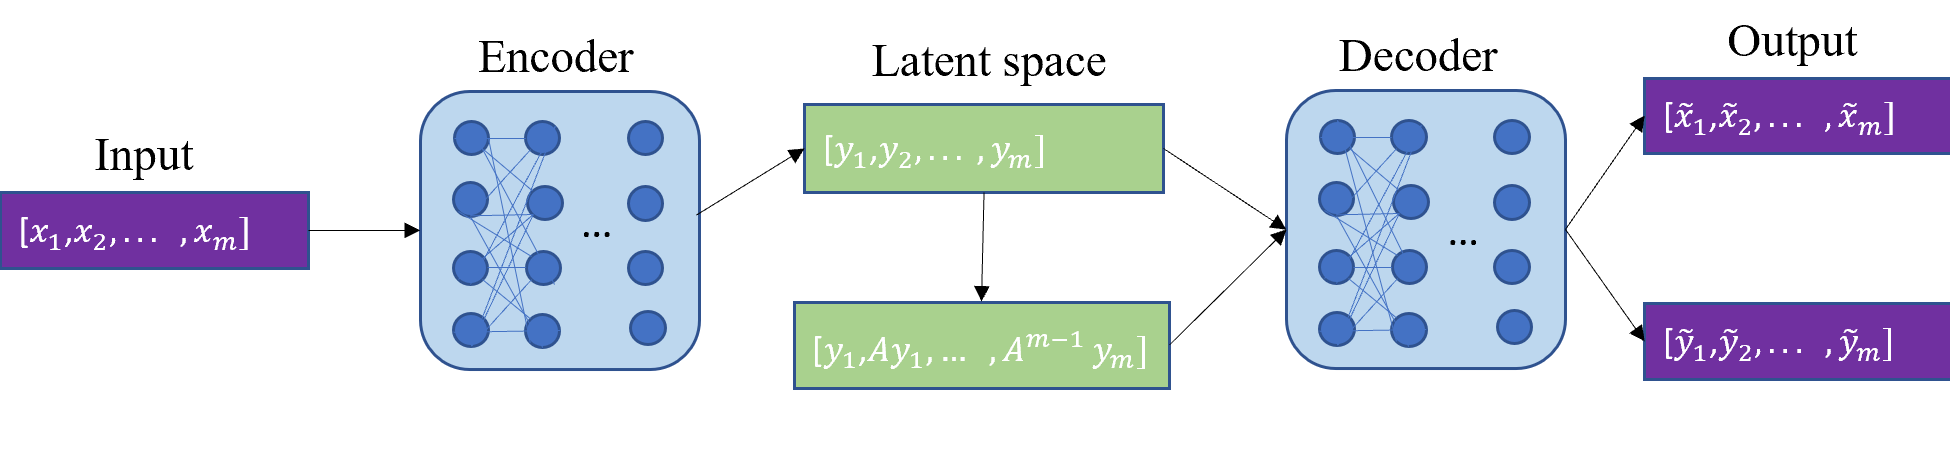
\includegraphics[width=\linewidth]{network_arc_pp_crop.PNG}
        \vspace{-8pt}
        \caption{Simple DMD autoencoder architecture. } 
    \end{figure}
    \vspace{-\intextsep}
    
    Figure 1 is an illustration of the simple DMD autoencoder architecture. The input time sequential data-set $X$ is passed to the encoder which is a nonlinear mapping $g$. The encoder output is called the latent space $y_{k} = g(x_{k})$. The latent space $Y$ is predicted by the Dynamic Mode Decomposition, $\tilde_{y_{k+1}} = A^{k}y_{0}$. Both the latent space $Y$ and predicted latent space $\tilde{Y}$ are passed to the decoder $g^{-1}$. Lastly, the decoder outputs $g^{-1}(Y)$ and $g^{-1}(\tilde{Y})$.
    
    The simple DMD autoencoder loss function is a combination of three evaluations: 
    
    1. Autoencoder reconstruction loss -  This ensures that the original state can be recovered.
    \begin{equation} \label{eq:8}
    L_{1} = MSE \left\| x_{0} - \tilde{x_{0}} \right\|
    \end{equation}
    
    2. DMD loss - evaluate the linearity of the latent space dynamics. The following is derived in equation (6).
    
    \begin{equation} \label{eq:9}
    L_{2} = \left\| Y' ( I - V V^{T}) \right\| _{F}^{2}
    \end{equation}
    
    
    3. DMD reconstruction loss- evaluate the DMD least squares fit of the $A$ matrix. 
    \begin{equation} \label{eq:10}
    L_{3} = MSE\left\| Y - \tilde{Y} \right\| 
    \end{equation}
    
The final loss function is $L = \alpha_{1}L_{1} + \alpha_{2}L_{2} + \alpha_{3}L_{3}$. 

% \tikzstyle{block} = [draw, rectangle, 
%     minimum height=3em, minimum width=6em]
% \tikzstyle{sum} = [draw, circle, node distance=1cm]
% \tikzstyle{input} = [coordinate]
% \tikzstyle{output} = [coordinate]
% \tikzstyle{pinstyle} = [pin edge={to-,thin,black}]

% \begin{tikzpicture}[auto, node distance=2cm,>=latex']
%     % Simple DMD auto-encoder graph. 
%     \node [input, name=input] {};
%     \node [sum, right of=input] (input) {$x$};
%     \node [block, right of=input, node distance=4cm] (latent) {$Y$};
%     \node [block, below of=latent, node distance=2cm] (latent_pred) {$\tilde{Y}$};
%     \node [sum, right of=latent, node distance=4cm] (output1) {$\tilde{x}$};
%     \node [sum, below of=output1, node distance=2cm] (output2) {$g^{-1}(\tilde{Y})$};
%     % draw arrows between blocks. 
%     \draw [->] (input) -- node[name=u1] {encode $g$} (latent);
%     \draw [->] (latent) -- node[name=u2] {decode $g^{-1}$} (output1);
%     \draw [->] (latent) -- node[name=u3] {$A$} (latent_pred);
%     \draw [->] (latent_pred) -- node[name=u3] {decode $g^{-1}$} (output2);
% \end{tikzpicture}


\section*{\fontsize{15}{15} \textbf{Results}}
    The simple DMD autoencoder is tested on nonlinear dynamical systems. 
    
    \textbf{Example 1- Discrete spectrum}
    Consider a simple nonlinear discrete spectrum system, described in equation (11).  
    \begin{equation} \label{eq:11}
        \begin{array}{l}
            \dot{x_{1}} = \mu x_{1} \\
            \dot{x_{2}} = \lambda (x_{2} - x_{1}^{2})
        \end{array}
    \end{equation}
    Given the input data we measure the dynamic mode decomposition accuracy by equation (6) and (7). As a result, $L_{2} =  0.000327$ and $L_{3} = 5.055e-05$, whereas in the latent space data-set $\tilde(y)$, $L_{2} =  0.0003006$ and $L_{3} = 0.0002703$. While the DMD loss decreased, the predictability loss did not improve. There is more room for improvement by adjusting the network's hyper-parameters. 

    \textbf{Example 2- Pendulum}
    Consider the simple pendulum which is a nonlinear continuous spectra systems, described in equation (12).  
    \begin{equation} \label{eq:12}
        \begin{array}{l}
            \dot{x_{1}} = x_{2}\\
            \dot{x_{2}} = -\sin(x_{1})
        \end{array}
    \end{equation}
    Given the input data we measure the dynamic mode decomposition accuracy by equation (6) and (7). As a result, $L_{2} =  0.04363$ and $L_{3} = 0.00335$, whereas in the latent space data-set $\tilde y$, $L_{2} =  0.00018$ and $L_{3} = 2.588e-05$. These results show that the encoder network finds a mapping which the nonlinear dynamics become approximately linear. 
    
    \begin{figure}[H]
        \centering
        \vspace{-\intextsep}
        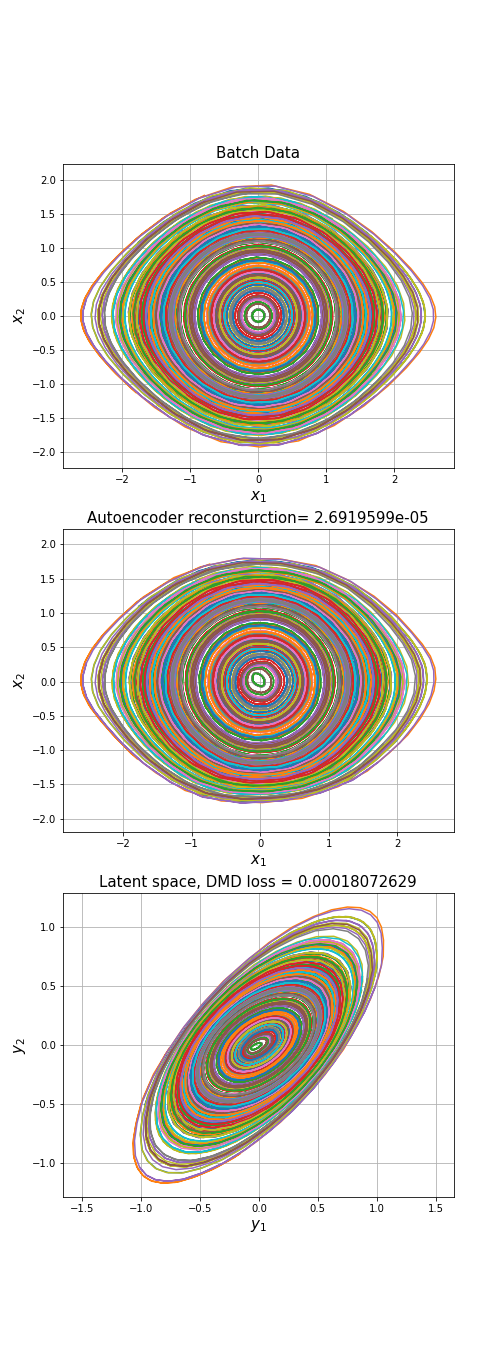
\includegraphics[width=\linewidth]{figure3.PNG}
        \vspace{-8pt}
        \caption{Figure 1a shows the phase portrait of the nonlinear pendulum. The simple DMD autoencoder attempts to reconstruct the input data and is shown in figure 1b. Figure 1c shows the dynamic mode decomposition reconstruction of the latent space. The simple DMD autoencoder does not account for continuous spectra and is used as a pretrain for the Koopman autoencoder developed by Lusch et al [{\color{blue} 1}]. This model is saved under \path{models/my_model_Ex2_oct21} and can be loaded easily, see \path{my_model_Ex2_oct21.ipynb}} 
    \end{figure}
    \vspace{-\intextsep}
        
\section*{\fontsize{15}{15} \textbf{Hyper-parameters}}
    Table 1 includes the DMD autoencoder network hyperparameters. The most important hyperparamters to adjust are the initial learning rate and learning scheduling. 
    \begin{tabular}{ |p{4cm}||p{2cm}|p{2cm}|  }
        \hline
         \multicolumn{3}{|c|}{Table 1} \\
         \hline
            \textbf{Hyper-parameters}  & \textbf{Discrete spectrum}  & \textbf{Pendulum} \\
            \hline
            Network layer type & Dense & Dense \\
            \hline
            Number of encoder hidden layers & 4 & 2 \\
            \hline
            Number of neurons in each layer & 32 & 80 \\
            \hline
            Latent dimension & 2 & 2 \\
            \hline
            Weight regularization method & L1 & L1 \\
            \hline 
            Weight regularization coefficient & 1e-2 & 1e-2\\
            \hline
            Hidden activation function & ELU & ELU\\
            \hline
            Output layer activation function & Linear & Linear\\
            \hline
            Weight initializer & he uniform & he uniform \\
            \hline
            Bias initializer & he uniform & he uniform \\
            \hline
            initial learning rate & 1e-3 & 1e-3 \\
            \hline 
            learning scheduling & 80 epoch & 80 epoch \\
        \hline 
    \end{tabular}

    Table 2 includes the loss coefficients used to train DMD autoencoder network. The corresponding coefficients relate to equation (8), (9), and (10). 
    \begin{tabular}{ |p{4cm}||p{2cm}|p{2cm}|  }
        \hline
        \multicolumn{3}{|c|}{Table 2} \\
        \hline
        \textbf{Loss function parameters}  & \textbf{Discrete spectrum} & \textbf{Pendulum} \\
        \hline
        \alpha_{1} & 1 & 1 \\
        \hline 
        \alpha{2} & 1 & 10 \\
        \hline 
        \alpha{3} & 1 & 1 \\
        \hline
    \end{tabular}

    Table 3 includes the parameters used to create the datasets. The code to generate the data is under 
    \path{data/data_class} and \path{data/data_maker}. 
    \begin{tabular}{ |p{4cm}||p{2cm}|p{2cm}|  }
        \hline
        \multicolumn{3}{|c|}{Table 3} \\
        \hline
        \textbf{Data-set parameters}  & \textbf{Discrete spectrum}  & \textbf{Pendulum} \\
        \hline
        Number of initial conditions in training data & 8000 & 8000 \\
        \hline 
        Number of initial conditions in testing data & 2000 & 2000 \\
        \hline 
        initial condition range x_{1} & [-0.5, 0.5] & [-1.8, 1.8] \\
        \hline 
        initial condition range x_{2} &  [-0.5, 0.5] & [-1.2, 1.2]\\
        \hline 
        Batch size & 256 & 256 \\
        \hline
        \hline
    \end{tabular}






 
    
\section*{\fontsize{15}{15} \textbf{Summary and Discussion}}
    In this report, we have analyzed the performance of the simple dynamic mode decomposition autoencoder on two different nonlinear dynamical systems. The model successfully learns a nonlinear mapping $g$ where dynamics are approximately linear. Next research steps are to test this model on a strongly nonlinear dynamical system simulation data-set that has noise. 

    
\section*{\fontsize{15}{15} \textbf{Code Availability}}
    The code used to generate these results is available at \url{https://github.com/opaliss/dmd_autoencoder} 

\begin{thebibliography}{9}

    \bibitem{Lusch} 
    Bethany Lusch, J. Nathan Kutz, and Steven L. Brunton. Deep learning for universal linear embeddings of nonlinear dynamics. Nature Communications, 9(1):4950, 2018.
    
    \bibitem{Tu}
    J. H. Tu, C. W. Rowley, D. M. Luchtenburg, S. L. Brunton, and J. Nathan Kutz. On dynamic mode decomposition: theory and applications. J. Comp. Dyn., 1(2):391-421, 2014. 

\end{thebibliography}

\end{document}
